\documentclass[notes]{subfiles}

\begin{document}
	\addcontentsline{toc}{section}{4.3 - The Fundamental Theorem of Calculus}
	\refstepcounter{section}
	\fancyhead[RO,LE]{\bfseries \large\nameref{cs43}} 
	\fancyhead[LO,RE]{\bfseries \currentname}
	\fancyfoot[C]{{}}
	\fancyfoot[RO,LE]{\large \thepage}	%Footer on Right \thepage is pagenumber
	\fancyfoot[LO,RE]{\large Chapter 4.3}
	
\section*{The Fundamental Theorem of Calculus}\label{cs43}
	\subsection*{Before Class}
	\addcontentsline{toc}{subsection}{Before Class}
	\subsubsection*{The First Fundamental Theorem}
	\addcontentsline{toc}{subsubsection}{The First Fundamental Theorem}
		\begin{ex}
			The function $f$ is given in the graph below.  Define the function $g(x)$ by the equation $g(x) =\ds \int_0^x f(t)\, dt$.  Find $g(0)$, $g(1)$, $g(2)$, and $g(3)$.  Then, sketch a rough graph of $g$ on the interval $[0,3]$.
			\begin{flushleft}
				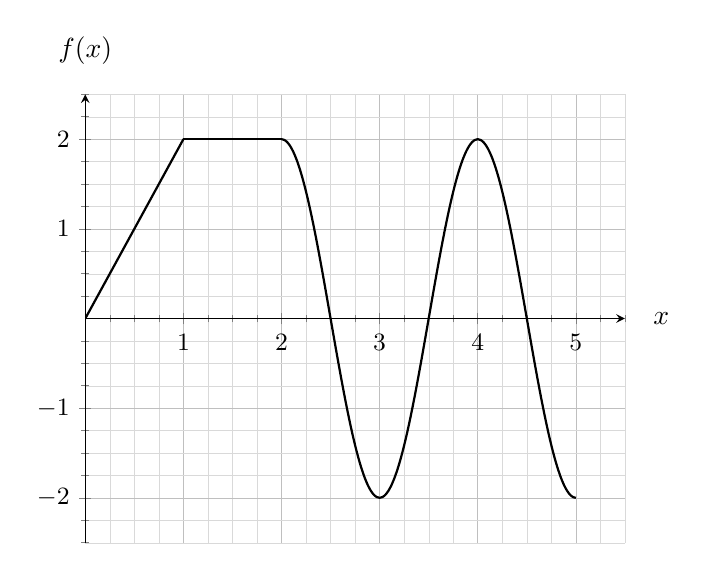
\begin{tikzpicture}
					\begin{axis}[
						grid=both,
						grid style={line width=.1pt, draw=gray!30},
						major grid style={line width=.2pt,draw=gray!50},
						every tick label/.append style={font=\small},
						axis x line = middle,
						axis y line = middle,
			    			every axis y label/.style={at={(ticklabel cs:1.15)}},
			    			%ytick = {-4, -2, -3, -1, 1, 2, 3, 4},
						y label style={at={(axis description cs:0,1.15)},anchor=north},
			    			ylabel = {$f(x)$},
		    				every axis x label/.style= {at ={(ticklabel cs:1)}},
		    				%xtick = {-4,-3,-2,-1,1,2,3,4},
		    				x label style={at={(axis description cs:1.1,.5)},anchor=east},
		    				xlabel = {$x$},
		    				xmax = 5.5, ymin = -2.5, ymax = 2.5,
		    				minor tick num = 3
					]
					
						\addplot[thick,domain = 0:1] {2*x};
						\addplot[thick,domain = 1:2] {2};
						\addplot[thick,smooth,samples=100,domain = 2:5] {2*cos((180)*(x-2))};
					\end{axis}
				\end{tikzpicture}
			\end{flushleft}
		\end{ex}
			\vs{2}
			
		\begin{thm}[The Fundamental Theorem of Calculus, Part 1 (FTC1)]
			\showto{ins}{
				If $f$ is continuous on $[a,b]$, then the function $g$ defined by $g(x) = \ds \int_a^x f(t)\,dt$, for $a\leq x\leq b$, is \fbox{continuous on $[a,b]$, differentiable on $(a,b)$, and $g'(x) = f(x)$}.  Using Leibniz notation, we have
					\[\dfrac{d}{dx}\left[\int_a^x f(t)\,dt\right] = f(x)\]
			}
			\showto{st}{
				If $f$ is continuous on $[a,b]$, then the function $g$ defined by $g(x) = \ds \int_a^x f(t)\,dt$, for $a\leq x\leq b$, is\vspace{25pt} \blank{6}\\ \\ \blank{1.5}.  Using Leibniz notation, we have\vspace{.75in}
			}
		\end{thm}
			\newpage
			
		\begin{ex}
			Find the derivative of the function $g(x) = \ds\int_0^x \sqrt{1-t^2}\,dt$.	
		\end{ex}
			\vs{1}
		\begin{ex}
			Find $\ds\dfrac{d}{dx}\int_1^{x^2}\csc t\,dt$
		\end{ex}
			\vs{1}
		
		\begin{ex}
			Find $F'(x)$, if $F(x) = \ds \int_x^0 \sqrt{1 + \sec y}\, dy$
		\end{ex}
			\vs{1}
			\newpage
			
	\subsubsection*{Pre-Class Activities}
	\addcontentsline{toc}{subsubsection}{Pre-Class Activities}
		\begin{ex}
			Let $g(x) = \ds \int_0^x f(t)\, dt$, where $f$ is the function in the graph below.\\
			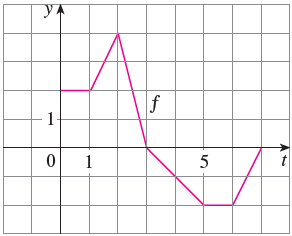
\includegraphics{4.3fig1}\\
			\begin{enumerate}[(a)]
				\item Evaluate $g(0), g(1), g(2), g(3)$, and $g(6)$.
					\vs{1}
					
				\item Where is $g$ increasing?
					\vs{1}
					
				\item Where does $g$ have a local max?
					\vs{1}
					
				\item Sketch a rough graph of $g$.
					\vs{2}
					
			\end{enumerate}
		\end{ex}	
			\newpage
			
		\begin{ex}
			Find the derivative of the following functions.
			\begin{enumerate}[(a)]
				\item $g(x) = \ds \int_2^x \sqrt{k + k^3}\, dk$
					\vs{1}
					
				\item $r(y) = \ds \int_y^2 t^3\cos t\, dt$
					\vs{1}
					
				\item $f(x) = \ds \int_0^{x^4} \tan^2t\, dt$
					\vs{1}
			\end{enumerate}
		\end{ex}
		
		\begin{ex}
			If $f(x) = \ds \int_0^x (1-t^2)\cos^2 t\, dt$, on what interval is $f$ increasing?
		\end{ex}
			\vs{1}
			\newpage
			
	\subsection*{In-Class}
	\addcontentsline{toc}{subsection}{In-Class}
	\subsubsection*{The Second Fundamental Theorem}
	\addcontentsline{toc}{subsubsection}{The Second Fundamental Theorem}	
		\begin{thm}[The Fundamental Theorem of Calculus, Part 2 (FTC2)]
			\showto{ins}{
				If $f$ is \textbf{continuous} on $[a,b]$, then $\ds \int_a^b f(x)\, dx = F(b)-F(a)$, where \fbox{$F$ is any antiderivative of}\\ \fbox{$f$}.		
			}
			\showto{st}{
				If $f$ is \blank{1.5} on $[a,b]$, then\vspace{.75in}\\ where $F$ is \blank{3}.
			}
		\end{thm}
		\begin{ex}
			Evaluate $\ds \int_{-2}^1 x^3\,dx$
		\end{ex}
			\vs{1}
			\newpage
			
		\begin{ex}
			Find the area under the curve $y = x^2$ from 0 to 1.
		\end{ex}
			\vs{1}
			
		\begin{ex}
			Find the area under the curve $y = \sin x$, from $0$ to $\dfrac{3\pi}{2}$
		\end{ex}
			\vs{1}
			
		\begin{ex}
			Is the statement $\ds \int_{-1}^1 \dfrac{1}{x^3}\, dx = 0$ correct?  Why or why not?
		\end{ex}
			\vs{1}
			\newpage
	
		\begin{ex}
			Find the derivative of $g(r) = \ds \int_5^r (t-t^2)^8\,dt$
		\end{ex}
			\vs{1}
			
		\begin{ex}
			Find the derivative of $R(y) = \ds \int_{y}^4 t^5\sec t\, dt$
		\end{ex}
			\vs{1}
			
		\begin{ex}
			Find the derivative of $y = \ds\int_0^{4x^3} \tan^2\theta\, d\theta$
		\end{ex}
			\vs{1}
			\newpage
			
		\begin{ex}
			Calculate the integral $\ds \int_1^3 (x^2+2x-4)\, dx$
		\end{ex}
			\vs{1}
			
		\begin{ex}
			Calculate the integral $\ds \int_0^2 \lrpar{\dfrac{4}{5}t^3-\dfrac{3}{4}t^2+\dfrac{2}{5}t}\,dt$
		\end{ex}
			\vs{1}
			
		\begin{ex}
			Calculate the integral $\ds \int_1^9 \sqrt{x}\,dx$
		\end{ex}
			\vs{1}
			\newpage
			
		\begin{ex}
			Calculate the integral $\ds \int_1^4 \dfrac{2+x^2}{\sqrt{x}}\,dx$
		\end{ex}
			\vs{1}
			
		\begin{ex}
			Calculate the integral $\ds \int_{\pi/6}^{\pi/2}\csc t\cot t\, dt$
		\end{ex}
			\vs{1}
			
		\begin{ex}
			Calculate the integral $\ds \int_{-1}^2 (3u-2)(u+1)\, du$
		\end{ex}
			\vs{1}
			\newpage
			
		\begin{ex}
			Calculate the integral $\ds \int_{\pi/4}^{\pi/3} \csc^2\theta\, d\theta$
		\end{ex}
			\vs{1}
			
		\begin{ex}
			Calculate the integral $\ds \int_1^{18} \sqrt{\dfrac{2}{z}}\, dz$
		\end{ex}
			\vs{1}
			
		\begin{ex}	
			Evaluate the integral $\ds \int_1^2 \dfrac{v^5+3v^6}{v^4}\, dv$
		\end{ex}
			\vs{1}
			\newpage
			
		\begin{ex}
			Evaluate the integral $\ds\int_0^\pi f(x)\, dx$, where $f(x) = \begin{cases}\sin x & \text{if }0\leq x < \pi/2 \\ \cos x & \text{if }\pi/2\leq x\leq \pi \end{cases}$
		\end{ex}
			\vs{1}
			
		\begin{ex}
			Evaluate the limit $\ds \lim_{n\to \infty} \sum_{i=1}^n \lrpar{\dfrac{i^4}{n^5} + \dfrac{i}{n^2}}$.  \emph{Hint}: Consider it as a Riemann sum on $[0,1]$.
		\end{ex}
			\vs{1}
		
		\begin{ex}
			If $f(1) = 12$, $f'$ is continuous, and $\ds \int_1^4 f'(x)\, dx = 17$, what is the value of $f(4)$?
		\end{ex}	
			\vs{1}
			\newpage
	
	\subsection*{After Class}
	\addcontentsline{toc}{subsection}{After Class}
		\begin{ex}
			Compute $\ds \int_0^1 (1+r)^3\, dr$
		\end{ex}
			\vs{1}
			
		\begin{ex}
			Find the area under the curve $f(x) = \dfrac{x^4 + 1}{x^2}$ between 1 and 2.
		\end{ex}
			\vs{1}

		\begin{ex}
			Evaluate $\ds \int_{-1}^1 x^{2022}\, dx$
		\end{ex}
			\vs{1}
			
		\begin{ex}
			What does it mean for differentiation and integration to be inverse processes?
		\end{ex}
			\vs{1}
	\clearpage	
\end{document}